\chapter{Modelli e formulazioni matematiche}

\section{The Traveling Salesman Problem}
Il Traveling Salesman Problem (TSP) � il problema pi� noto dell'ottimizzazione combinatoria.
Siano date $n$ citt� e i costi $c_{ij}$ per andare dalla citt� $i$ alla citt� $j$.
Si vuole determinare un cammino che parte da una citt� (diciamo $i_{1}$), visitare una ed una sola volta tutte le rimanenti citt� e terminare nella citt� di partenza $i_{1}$.
Inoltre si vuole che il costo di tale cammino sia minimo.\newline
Ha molteplici applicazioni pratiche e teoriche perche � la struttura di molti problemi pratici.\newline
Si � soliti modella il TSP come segue:
\begin{itemize}
	\item � dato un grafo orientato (o non orientato) $G = (N,A)$
	dove $N$ � un insieme di $n$ vertici e $A$ � un insieme di $m$ archi.
	
	Ad ogni arco $\emph{(i,j)} \in \emph{A}$ � associato un costo $c_{ij}$.
	
	Un circuito hamiltoniano di $G$ � un circuito che passa per ogni vertice una ed una sola volta.\newline
	Il costo di un circuito hamiltoniano di $G$ � pari alla somma dei costi degli archi che compongono il circuito;
	\item il problema del TSP � di trovare un grafo $G$, con una data matrice dei costi [$c_{ij}$], un circuito hamiltoniano di costo minimo.
\end{itemize}

\section{Formulazioni Matematiche del TSP}
In letteratura esistono molteplici (e a volte fantasiose) formulazioni del TSP.\newline
Presentiamo le due formulazioni pi� note e su cui si basano i metodi esatti pi� efficienti.

\subsection{TSP asimmetrico}
I costi $c_{ij}$ non verificano $c_{ij} = c_{ji}\;\forall\;i,j$ con $i < j$.\newline
Sia $x_{ij}$ una variabile $(0-1)$ associata ad ogni arco $(i,j) \in A$ dove $x_{ij}=1$ se l'arco $(i,j)$ � nella soluzione ottima e $x_{ij}=0$ altrimenti.\newline

\begin{equation}
	Min\;\;\displaystyle\sum_{i\in N}^{} \sum_{j\in N}^{} c_{ij} x_{ij}
\end{equation}
\begin{equation}
	s.t.\;\;\displaystyle\sum_{i\in N}^{} x_{ij} = 1,\;\;\forall j \in N
\end{equation}
\begin{equation}
	\;\;\;\;\;\;\;\displaystyle\sum_{j\in N}^{} x_{ij} = 1,\;\;\forall i \in N
\end{equation}
\begin{equation}
	\;\;\;\;\;\;\;\;\;\;\;\;\;\;\;\;\;\;\displaystyle\sum_{i\in S}^{} \sum_{j\in N\setminus S}^{} x_{ij} \ge 1,\;\;\forall S \subset N
\end{equation}
\begin{equation}
	\;\;\;\;\;\;\;\;\;\;x_{ij} \in \{0,1\}\;,\;\forall (i,j) \in A
\end{equation}

Il vincolo $1.4$ impone che ogni soluzione ammissibile debba contenere almeno un arco $(i,j)$ con $i\in S$ e $j\in N\setminus S$ per ogni sottoinsieme $S$ di $N$.
Un'alternativa al vincolo $1.4$ �:
\begin{equation}\tag{1.4'}
\;\;\;\;\;\;\;\;\;\;\;\;\;\;\;\;\;\;\displaystyle\sum_{i\in S}^{} \sum_{j\in S}^{} x_{ij} \le |S| - 1,\;\;\forall S \subset N
\end{equation}

\subsection{TSP simmetrico}
Sia dato un grafo non-orientato $G=(N,A)$ con $c_{ij} = c_{ji}\:,\forall i,j\in N$.\newline
Gli archi di $A$ sono numerati da $1$ a $m$. L'arco di indice $l$ corrisponde a $(\alpha_{l},\beta_{l})$ con $\alpha_{l} < \beta_{l}$.\newline
$A_{i}$ � il sottoinsieme degli indici degli archi che incidono sul vertice $i$:
\begin{center}
	$A_{i} = \{l:\;l=1,m\;\;s.t.\;\alpha_{l}=i\;or\;\beta_{l}=i\}$
\end{center}

Per una dato $S\in N$ e $\bar{S} = N\setminus S$ indichiamo con $(S, \bar{S})$ il sottoinsieme degli indici degli archi per cui $\alpha_{l}\in S$ e $\beta_{l}\in \bar{S}$ oppure $\alpha_{l}\in \bar{S}$ e $\beta_{l}\in S$.

Ad ogni arco di incide $l$ � associato un costo $d_{l}=c_{\alpha_{l}\beta_{l}}$ e $x_{l}\in \{0,1\}$ � una variabile che vale 1 se e solo se l'arco di indice $l$ � nella soluzione ottima.
\begin{equation}
	Min\;\;\displaystyle\sum_{l=1}^{} d_{l}\:x_{l}
\end{equation}
\begin{equation}
	s.t.\;\;\displaystyle\sum_{l\in A_{i}}^{} x_{l}=2,\; \forall i\in N
\end{equation}
\begin{equation}
	\;\;\;\;\;\;\;\;\;\displaystyle\sum_{l\in (S, \bar{S})}^{} x_{l} \ge 1,\;\forall S \subset N
\end{equation}
\begin{equation}
	x_{l}\in \{0,1\},\;\;l=1,...,m
\end{equation}

\subsection{Eliminazione subtours di Miller, Tucker, Zemlin (1960)}
Sia $u_{i}$ una variabile intera il cui valore sappresenta la posizione che il vertice $i$ occupa nel tour.

\begin{center}
	Es. tour (1,4,5,3,2,1) per TSP con n=5 vertici, si ha $u_{1}=1,\;u_{2}=5,\;u_{3}=4,\;u_{4}=2,\;u_{5}=3$	
\end{center}

Miller, Tucker e Zemlin propongono in alternativa a:
\begin{equation}\tag{*}
	\displaystyle\sum_{i\in S}^{}\sum_{j\in N\setminus S}^{} x_{ij} \ge 1,\;\;\forall S\subset N
\end{equation}
hanno imposto i seguenti vincoli:
\begin{equation}
	u_{i}-u_{j}+nx_{ij}\le n-1,\;\; i=1,...,n\:,\;j=2,...,n
\end{equation}
Ogni tour hamiltoniano soddisfa questi vincoli e ogni subtour li viola.\newline
\begin{wrapfigure}[5]{l}{0.5\textwidth}
	\vspace{-2em}
	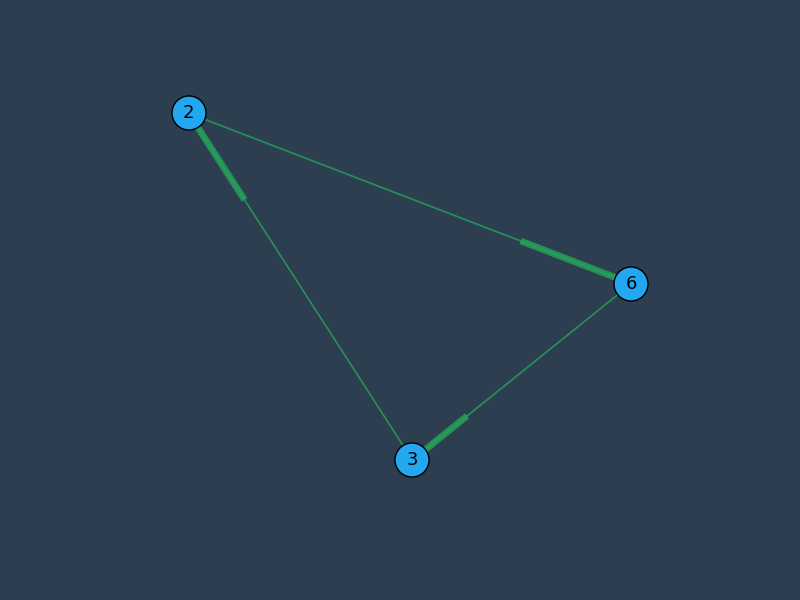
\includegraphics[height=5cm]{images/graph1.png}
	\caption{Grafo orientato}
\end{wrapfigure}
\begin{description}
	\vspace{1.5em}
	\item $u_{2}-u_{6}+n\;\cdot x_{2,6}\le n-1$
	\item $u_{6}-u_{3}+n\;\cdot x_{6,3}\le n-1$
	\item $u_{3}-u_{2}+n\;\cdot x_{3,2}\le n-1$
	\item {\hskip 5.6em}$\downarrow$
	\item {\hskip 3em}$3n \le 3(n-1)$
\end{description}\newpage

\subsection{Il Traveling salesman problem con time windows (TSPTW)}

� una variante del TSP che ha molte applicazioni.

Sia dato un grafo orientato $G=(V,A)$ di $n+1$ vertici $(V=\{0,1,...,n\})$.

Ad ogni arco $(i,j)\in A$ sono associati
\begin{itemize}
	\item un costo $c_{ij} \ge 0$
	\item un tempo di percorrenza $\theta_{ij}\ge 0$
\end{itemize}
Ad ogni vertice � associato un intervallo $[r_{i},d_{i}]$ chiamato "time window" che rappresenta l'orario in cui il vertice $i$ pu� essere vistato dal "salesman".

Ovvero il salesman pu� visitare $i$ ad ogni tempo $t\in \mathbb{Z}^{+}$ con $r_{i}\le t\le d_{i}$.\newline
Il problema consiste nel trovare una sequenza dei vertici di $G$ che parte dal vertice $0$ al tempo $0$ e finisce al nodo $0$ tale che sia il minimo il costo del circuito e il tempo di arrivo al nodo $i$ sia nell'intervallo $[r_{i},d_{j}],\;\forall i\in V$.\newline
Si consideri la sequenza $(0,i,..,i_{k-1},i_{k},...,i_{n},0)$ e sia $t_{i_{k}}$ il tempo di arrivo al vertice $i_{k},\; k=0,1,...,n+1$.

I tempi di arrivo sono calcolati come:
\begin{equation}
	t_{0}=0
\end{equation}
\begin{equation}
	t_{i_{k}}=\max \{t_{i_{k-1}}+\theta_{i_{k-1}}\cdot i_{k},\; r_{i_{k}}\}
\end{equation}


\subsubsection{Formulazione del TSPTW}
Sia $x_{ij}$ una variabile binaria intera che assume il valore $1$ se il vertice $i$ � visitato immediatamente prima di $i$ e $x_{ij}=0$ altrimenti.
\begin{flalign}
	& Min\;\;\displaystyle\sum_{(i,j)\in A}^{}c_{ik}x_{ij} \\
	& s.t.\;\;\;\;\displaystyle\sum_{i\in A_{j}^{-}}^{}x_{ij}=1,\;\;\forall j\in V \\		
	& \;\;\;\;\;\;\;\;\displaystyle\sum_{j\in A_{i}^{+}}^{}x_{ij}=1,\;\;\forall i\in V \\
	& \;\;\;\;\;\;\;\;t_{i}+\theta_{ij}-t_{j}\le M(1-x_{ij},\;\;\forall (i,j)\in A,\; j\ne 0) \\
	& \;\;\;\;\;\;\;\;t_{i}\le d_{i},\;\;\forall i\in V \\
	& \;\;\;\;\;\;\;\;t_{i}\ge r_{i},\;\;\forall i\in V \\
	& \;\;\;\;\;\;\;\;x_{ij}\in \{0,1\},\;\;\forall \in A \\
	& \;\;\;\;\;\;\;\;t_{i}\in \mathbb{N}^{+},\;\;\forall i\in V
\end{flalign}

dove 
\begin{flalign*}
	& A_{i}^{+}=\{j\in V:(i,j)\in A\} \\
	& A_{i}^{-}=\{j\in V:(i,j)\in A\} \\
	& M\;�\;un\;intero\;grande\;a\;piacere \\
	& r_{0}=d_{0}=0
\end{flalign*}

\section{Project scheduling with resource constraints (PSR)}
\`E dato un insieme $\mathbb{X}=\{1,...,n\}$ di $n$ jobs.

Sono disponibili $m$ risorse dove ogni risorsa $k$ ha una disponibilit� $b_{k}$ ad ogni istante del periodo di scheduling.

Ogni job $i$ ha un tempo di processo $d_{i}$ e la sua esecuzione, una volta iniziata, non pu� essere interrotta.

Il job $i$ per essere eseguito richiede $b_{ik}$ unit� della risorsa $k$ per ciascun intervallo di tempo in cui rimane in esecuzione.\newline
\`E dato un grafo $G=(X,H)$ di precedenze, dove ogni arco $(i,j)\in H$ impone che il job $j$ pu� iniziare solo dopo che il job $i$ � stato completato.

\begin{itemize}
	\item Si vuole determinare il tempo di inizio di processo di ogni job in modo che siano soddisfatti i vincoli di precedenza, i vincoli sulle risorse e sia minima la durata complessiva del progetto
\end{itemize}

\subsection{Esempio di PSR}
Siano dati $n=11$ jobs e $m=3$ risorse con $b_{1}=b_{2}=b_{3}=4$ e un grafo $H$ delle precedenze corrispondenti agli archi della figura ~\ref{fig:grafoHDellePrecedenze}.

Si osservi che i jobs $2$ e $3$ non possono essere eseguiti in parallelo poich� $r_{2,1}+r_{3,1}=5 > b_{1}$!

\begin{figure}[h]
	\centering
	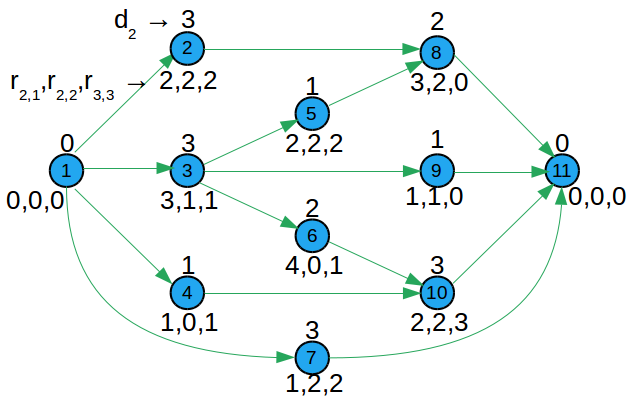
\includegraphics[height=6.5cm]{images/graph2.png}
	\caption{Grafo H delle precedenze}
	\label{fig:grafoHDellePrecedenze}
\end{figure}